\documentclass{article}

\usepackage{graphicx}
\usepackage{tikz}
\usepackage{tikzsymbols}
\usetikzlibrary{calc,patterns,shapes.geometric}
\pagestyle{empty}
\usepackage[margin=0pt]{geometry}
\geometry{papersize={14in,12in}}

\def\centerarc[#1](#2)(#3:#4:#5){\draw[#1] ($(#2)+({#5*cos(#3)},{#5*sin(#3)})$) arc (#3:#4:#5);}

\begin{document}
	\begin{figure}
		\centering
		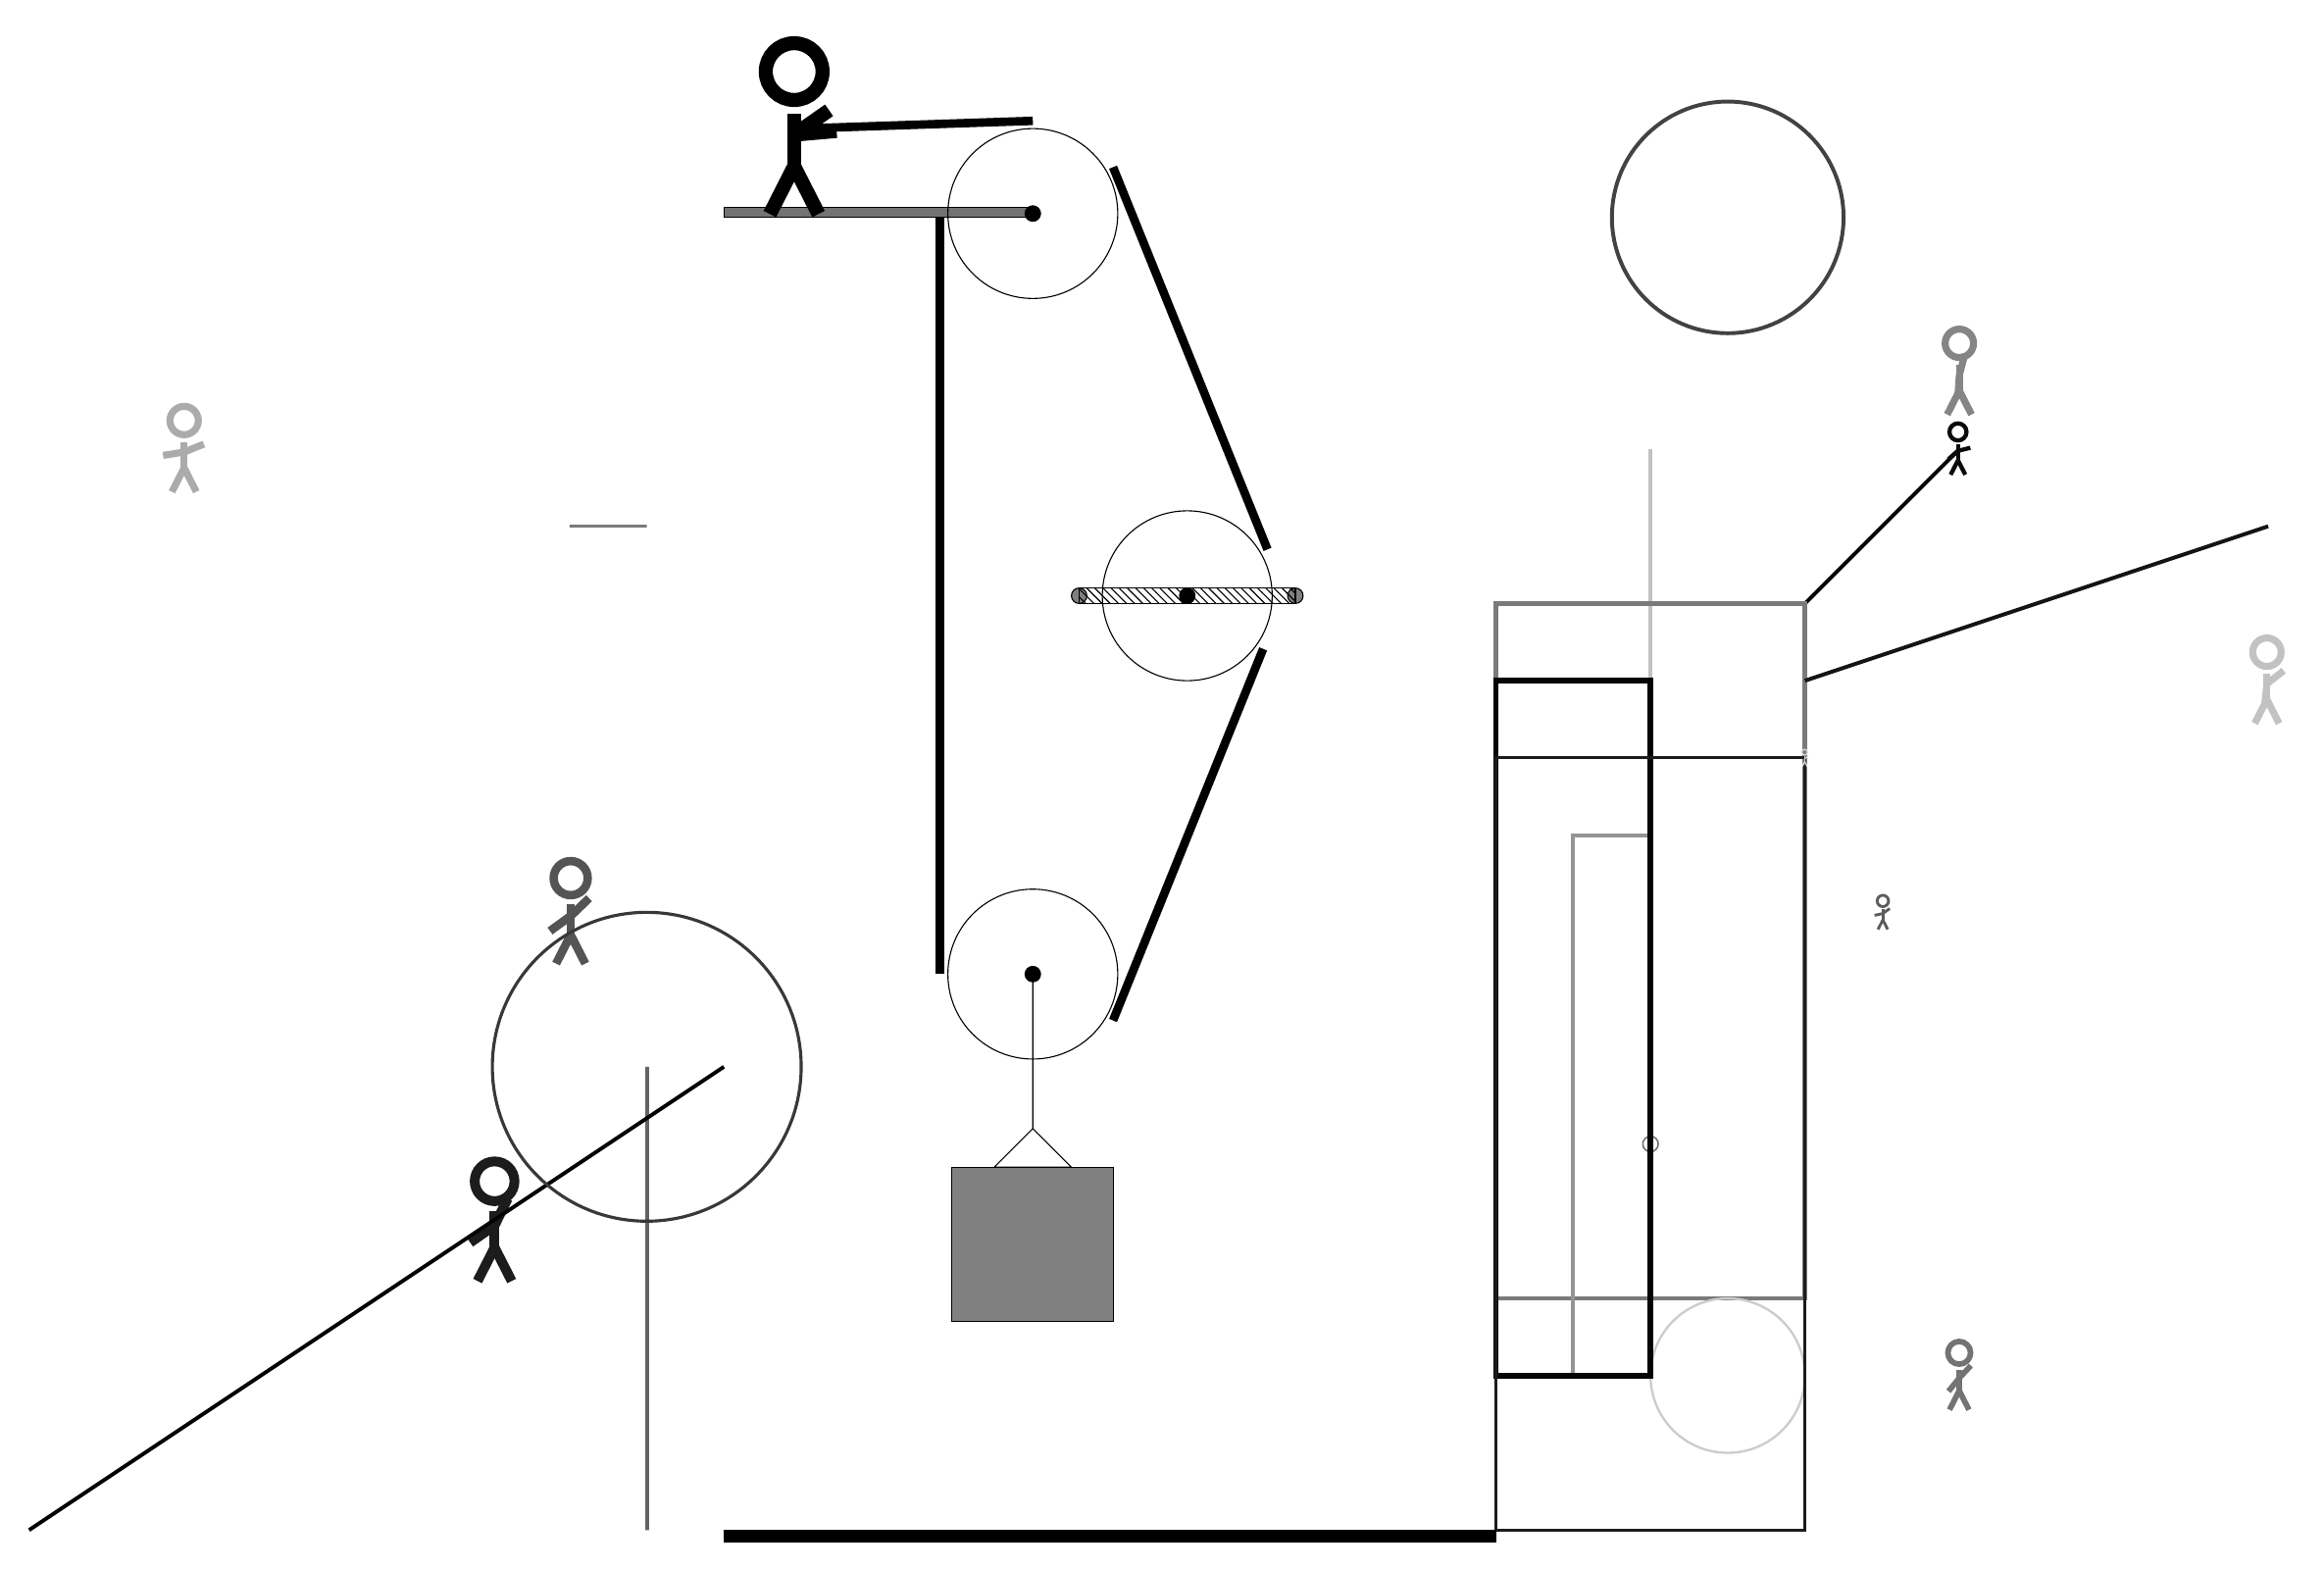
\begin{tikzpicture}
			%%%%% START %%%%%
			
			\draw[fill=black!55] (-2, 14) rectangle (2, 14.125);
			
			\draw (2, 4.2) circle (1.1);
			\draw[fill=black] (2, 4.2) circle (0.1);
			
			\draw (2, 14.05) circle (1.1);
			\draw[fill=black] (2, 14.05) circle (0.1);
			
			\draw[fill=white](4, 9.1) circle (1.1);
			\draw[fill=black] (4, 9.1) circle (0.1);
			\draw[fill=black!50] (2.6, 9.1) circle (0.1);
			\draw[fill=black!50] (5.4, 9.1) circle (0.1);
			\draw[pattern=north west lines, pattern color=black] (2.6, 9.2) rectangle (5.4, 9.0);
			
			\node[line width=0.4mm, color=black!64] at (13, 5) {\Strichmaxerl[2][12][36]};
			
			\draw[line width=0.3mm, color=black!58] (9, 6) rectangle (9, 0);
			\draw[line width=0.5mm, color=black!24](10, 11) -- (10, 2);
			\node[line width=0.6mm, color=black!67] at (-4, 5) {\Strichmaxerl[6][36][44]};
			
			\node[line width=0.2mm, color=black!89] at (-5, 1) {\Strichmaxerl[7][35][64]};
			
			\draw[line width=0.5mm, color=black!98](12, 9) -- (14, 11);
			
			\draw[line width=0.5mm, color=black!61] (-3, -3) rectangle (-3, 3);
			
			\draw[line width=0.6mm, color=black!52] (8, 9) rectangle (12, 0);
			\draw[line width=0.4mm, color=black!87] (8, 7) rectangle (12, 7);
			\draw [line width=0.2mm, color=black!56](10, 2) circle (0.1);
			\node[line width=0.3mm, color=black!24] at (18, 8) {\Strichmaxerl[5][84][38]};
			\draw[line width=0.5mm, color=black!92](12, 8) -- (18, 10);
			\draw [line width=0.5mm, color=black!74](11, 14) circle (1.5);
			\draw [line width=0.3mm, color=black!20](11, -1) circle (1.0);
			\draw[line width=0.5mm, color=black!42] (10, -1) rectangle (9, 6);
			\draw[line width=0.7mm, color=black!98] (8, -1) rectangle (10, 8);
			
			\node[line width=0.4mm, color=black!33] at (-9, 11) {\Strichmaxerl[5][9][22]};
			\draw[line width=0.5mm, color=black!99](-2, 3) -- (-11, -3);
			\draw[line width=0.4mm, color=black!52] (-4, 10) rectangle (-3, 10);
			
			\node[line width=0.2mm, color=black!96] at (14, 11) {\Strichmaxerl[3][41][14]};
			\draw[line width=0.4mm, color=black!89] (8, 7) rectangle (12, -3);
			
			\draw [line width=0.4mm, color=black!78](-3, 3) circle (2.0);
			\node[line width=0.4mm, color=black!48] at (14, 12) {\Strichmaxerl[5][86][75]};
			\node[line width=0.4mm, color=black!55] at (14, -1) {\Strichmaxerl[4][51][47]};
			\node[line width=0.5mm, color=black!16] at (12, 7) {\Strichmaxerl[1][88][37]};
			
			
			\draw (2, 4.2) -- (2, 2.2) -- (1.5, 1.7) -- (2.5, 1.7) -- (2, 2.2);
			\draw[fill=black!50] (0.95, 1.7) rectangle (3.05, -0.3);
			
			\draw[line width=1.1mm] (0.8, 14) -- (0.8, 4.2);
			\centerarc[line width=1.1mm](2, 4.2)(180:330:1.2000000000000002);
			\draw[line width=1.1mm](3.0392, 3.6) -- (4.983, 8.4117);
			\centerarc[line width=1.1mm](4, 9.1)(390:325:1.2000000000000002);
			\draw[line width=1.1mm](5.0392, 9.7) -- (3.0392, 14.65);
			\centerarc[line width=1.1mm](2, 14.05)(30:90:1.2000000000000002);
			\draw[line width=1.1mm](2, 15.25) -- (-1, 15.15);
			
			\node at (-1, 15.15) {\Strichmaxerl[10][-175][35]};
			
			\draw[fill=black] (-2, -3) rectangle (8, -3.15);
			
			%%%%% END %%%%%
		\end{tikzpicture}
	\end{figure}	
\end{document}